\subsection{Data List Interface}

The data list interface is used to display game records retrieved from the database in a structured table format. 
In this application, the main table shown to users is the \textit{Game List}, which presents important information about each game, including game ID, title, base price, release date, and developer name.

The data displayed in this interface is loaded dynamically from the MySQL database through the backend API. 
When the user opens or refreshes the page, the application sends a request to retrieve game records. 
The backend then queries the \texttt{GAME} table and joins it with the \texttt{DEVELOPER} table so that each game can be shown together with its developer name.

In addition to displaying all games, the interface also provides a search area where users can filter games by genre and maximum price. 
This feature is connected to the stored procedure \texttt{GetGamesByGenreAndPrice}, allowing the application to demonstrate data retrieval through a database-level stored procedure instead of filtering only on the frontend.

The interface helps users view database records more conveniently and confirms that the application can successfully retrieve and present relational data from the implemented database.

\begin{figure}[H]
    \centering
    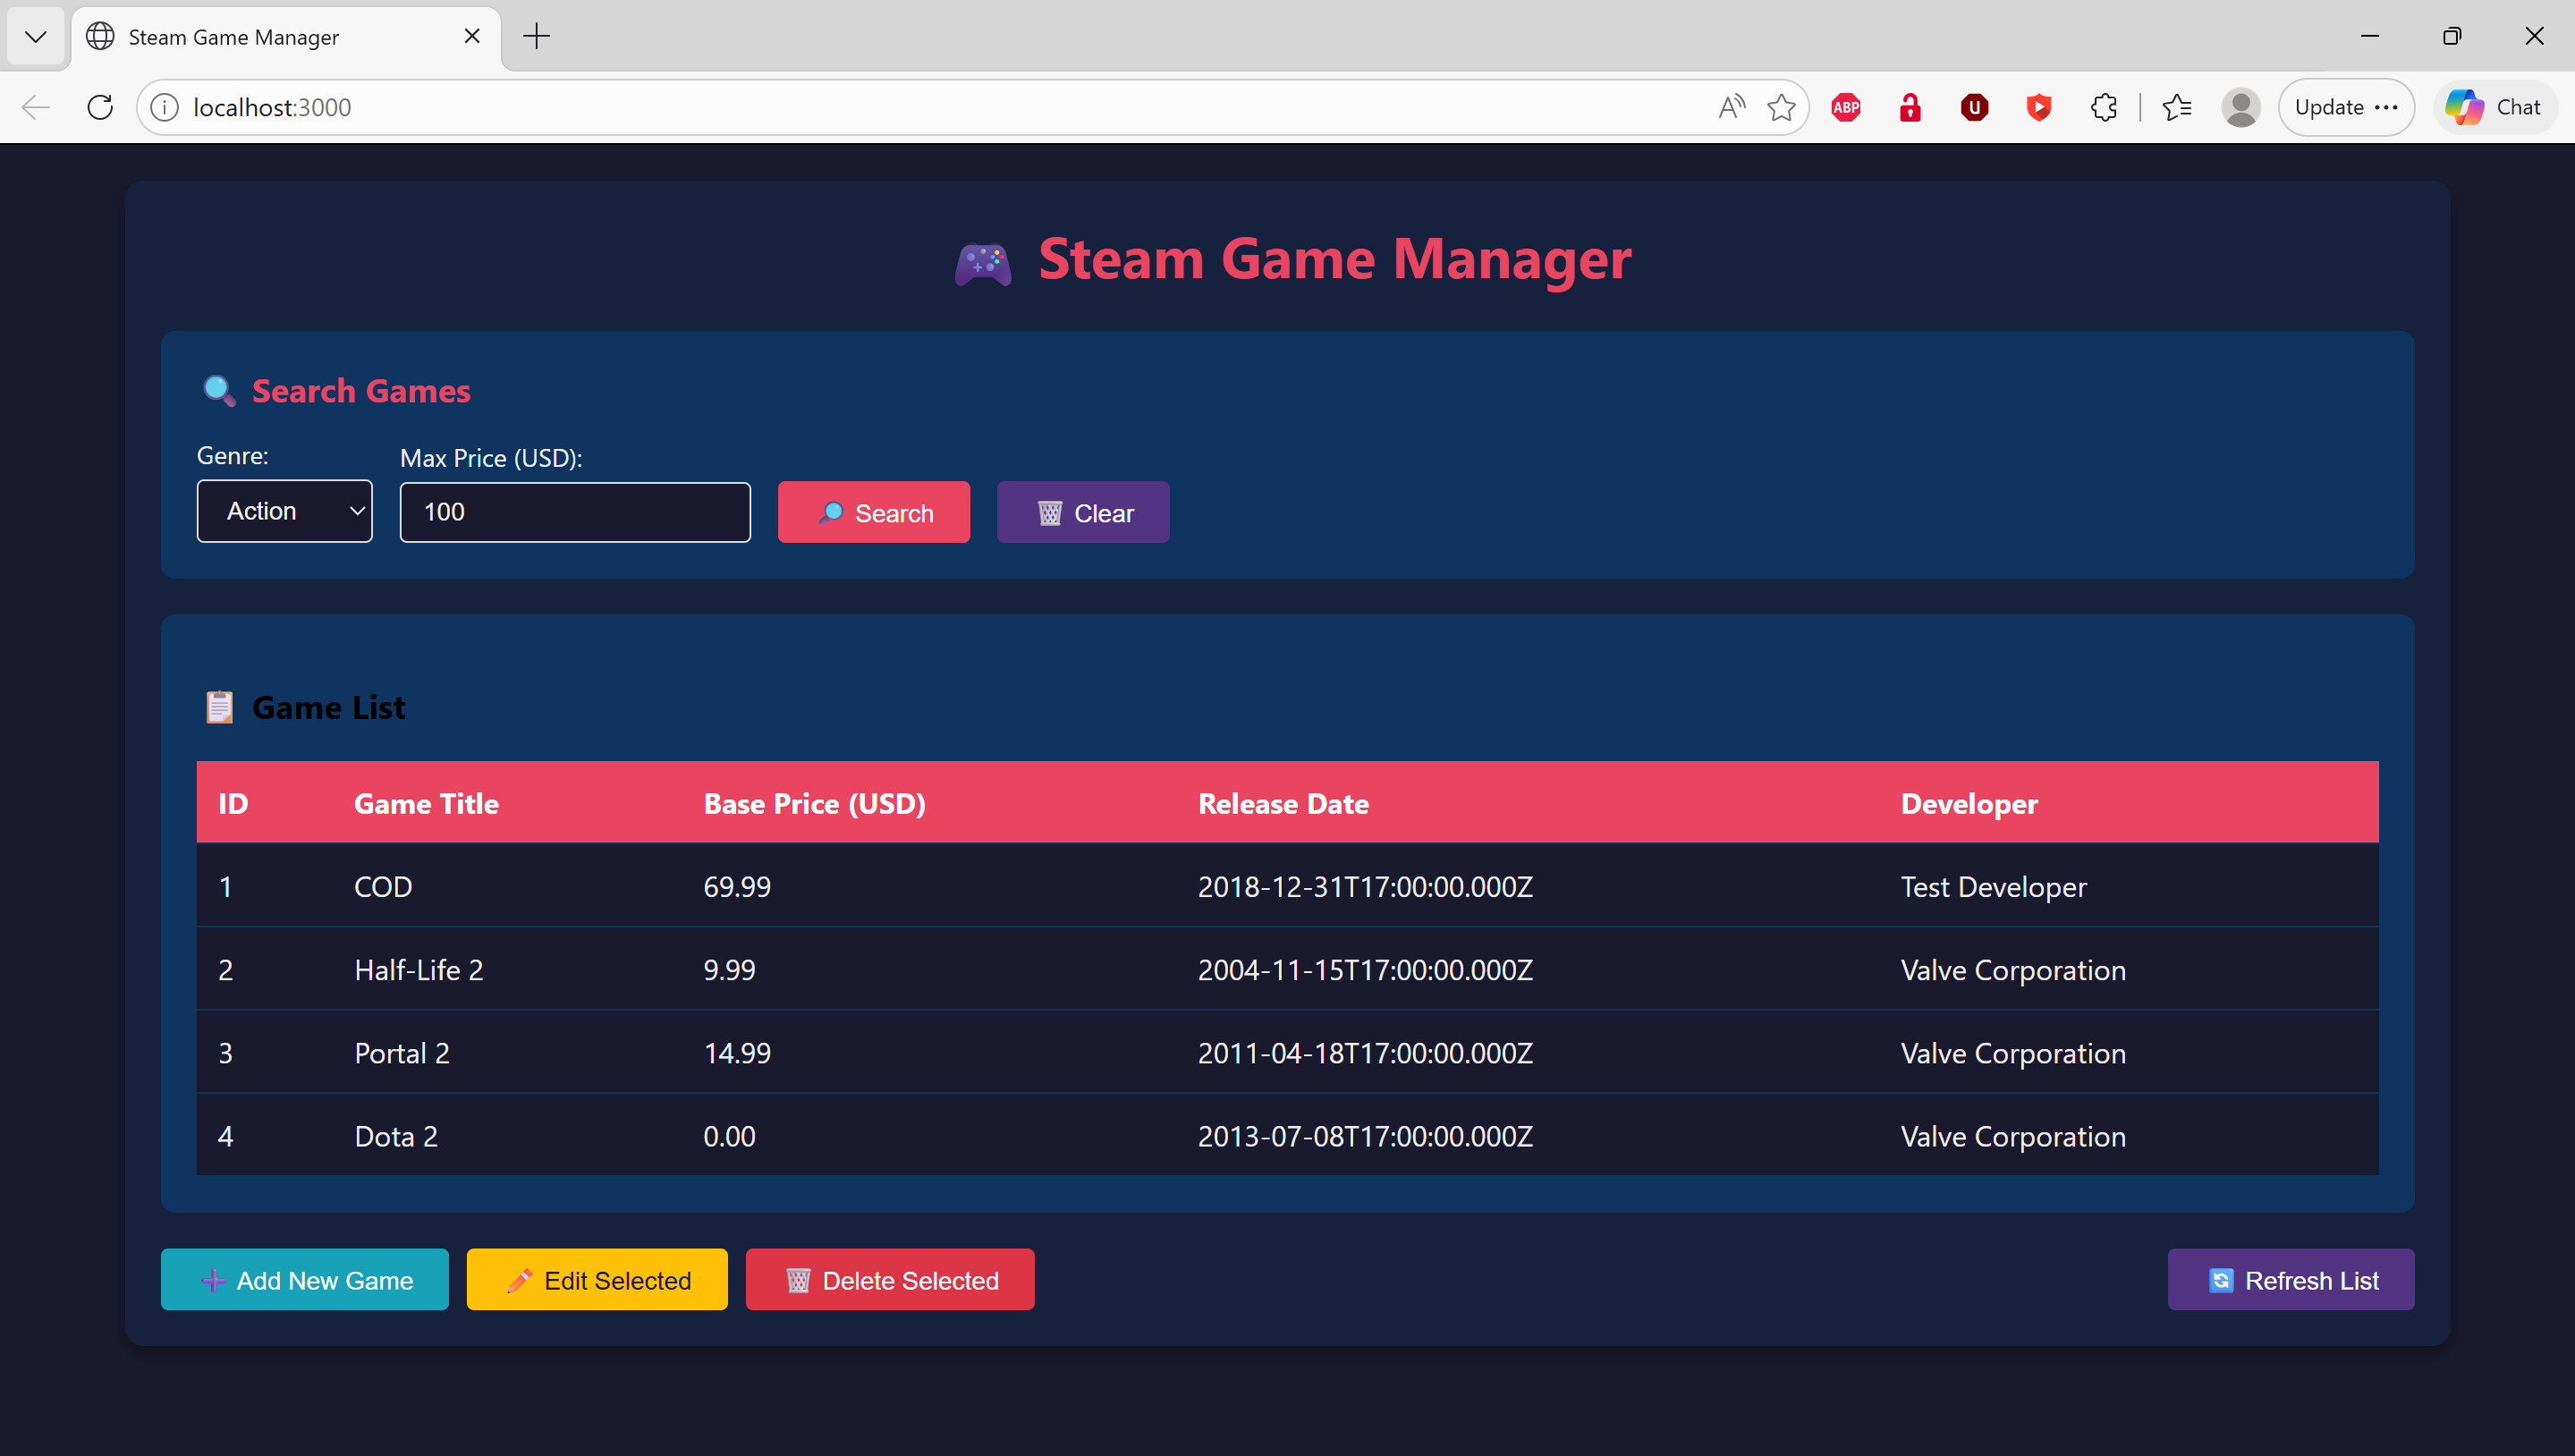
\includegraphics[width=0.95\linewidth]{graphics/data_list_interface.png}
    \caption{Data list interface displaying game records retrieved from the database}
    \label{fig:data-list-interface}
\end{figure}